\section{Evaluation}

%V.	Evaluation
%	a.	Models
%		i.	Model Accuracy
%			1.	Matlab
%		ii.	Performance/Overhead
%			1.	Tess
%				a.	Time to build the model
%				b.	Phase Change Reaction
%		i.	Video Application adding threads
%		ii.	Time to react to phase changes
%		iii.	Show model accuracy through transition?
%	b.	Decisions
%		i.	Decision Accuracy
%			1.	Matlab
%		ii.	Performance/Overhead
%			1.	Tess
%	c.	Dynamic System
%		i.	Single Application � right sizing
%			1.	Without phase changes
%			2.	With phase changes
%			3.	Baseline � all allocations
%			4.	Measure Energy
%		ii.	Video, Animation, and Throughput Applications w/o phase changes
%			1.	Show throughput and missed deadlines for all the possible mixes
%			2.	Is it possible to show optimal?
%			3.	What is the baseline?
%		iii.	Video, Animation, and Throughput Applications w/ phase changes
%			1.	Show throughput and missed deadlines for all the possible mixes
%			2.	Basically just to show the system works


\cite{tess09}
\cite{SPEC2006}
\cite{parsec}
\cite{dacapo}
\cite{lithe}
\cite{matlab}
\cite{cvx}
%\cite{pulse}
\cite{bates-aes03}

PULSE (Preemptive User-Level SchEduling)
Lithe (LIquid THrEads)

\subsection{Experimental Methodology}
\label{sec:Platform}

To evaluate \pacora, we use two different implementations of the framework on the same hardware platform.  Our offline framework was used to experiment with the accuracy of different types of models and test 

\fix{2 implementations}

\subsubsection{Experimental Platform}

We use a prototype version of Intel's Sandy Bridge x86
processor to collect results on resource allocation and application
co-scheduling.  By using a real hardware prototype, we are able to run
full applications for realistic time scales and workload sizes, while running a standard operating system.  The processor is similar
to the commercially available client chip, but with additional
hardware to support way-based cache partitioning in the LLC.

The Sandy Bridge client chip has four quad-issue out-of-order
superscalar cores, each of which supports two hyperthreads using
simultaneous multithreading~\cite{IntelRefManual:2011}.  Each core has
private \wunits{32}{KB} instruction and data caches, as well as a
\wunits{256}{KB} private non-inclusive L2 cache.  The LLC is a 12-way
set-associative \wunits{6}{MB} inclusive L3 cache, shared among all
cores using a ring-based interconnect.  All three cache levels are
write-back.  Larger server versions of the same processor family have
up to \wunits{15}{MB} of LLC capacity.

The cache partitioning mechanism is way-based and modifies the
cache-replacement algorithm.  Each core can be assigned a subset of
the 12 ways in the LLC.  Although all cores can hit on data stored in
any way, a core can only replace data stored in one of its assigned
ways.  Allocation of ways among cores can be completely private,
completely shared, or overlapping.  Data is not flushed when the way
allocation changes; newly fetched data will just be written into one
of the assigned ways according to the updated allocation
configuration.

We use a customized BIOS that enables the cache partitioning
mechanism,

To measure on-chip energy, we use the energy counters available on
Sandy Bridge to collect the energy used by the entire socket and also
the total combined energy of cores, their private caches, and the
LLC. The counters measure power
at a $1/2^{16}$ second granularity.

\subsection{Linux Analysis}

and run unmodified Linux-2.6.36 for all of our experiments.
We use the Linux {\tt taskset} command to pin each application to
subsets of the available HyperThreads.

To measure application performance, we use the \texttt{libpfm}
library~\cite{Eranian:OLS06,Perfmon2}, built on top of the
\texttt{perf\_events} infrastructure introduced in Linux 2.6.31, to
access various performance-monitoring counters available on the
machine~\cite{Intel:Manual2012}.

We access these counters using the Running Average Power Limit
(RAPL) interfaces~\cite{Intel:Manual2012}.

\subsubsection{Description of Workloads}

We built our workload using a wide range of codes from three different
popular benchmark suites: SPEC CPU 2006~\cite{SPEC2006},
DaCapo~\cite{Blackburn:OOSPLA2006}, and PARSEC~\cite{Bienia:PdD2011}.
We included some additional application benchmarks to broaden the
scope of the study, and some microbenchmarks that exercise certain
features of the system.

The \textbf{SPEC CPU 2006} benchmark suite~\cite{SPEC2006} is a
CPU-intensive, single-threaded benchmark suite, designed to stress a
system's processor, memory subsystem and compiler.  Using the
similarity analysis performed by Phansalkar et
al.~\cite{Phansalkar:ISCA2007}, we subset the suite, selecting 4
integer benchmarks (astar, libquantum, mcf, omnetpp) and 4
floating-point benchmarks (cactusADM, calculix, lbm, povray).  Based
on the characterization study by Jaleel~\cite{Jaleel:TR2007}, we also
pick 4 extra floating-point benchmarks that stress the LLC: GemsFDTD,
leslie3d, soplex and sphinx3.  When multiple input sets and sizes are
available, we pick the single \textit{ref} input indicated by
Phansalkar et al.~\cite{Phansalkar:ISCA2007}. SPEC is the only
benchmark suite used in many previous characterizations of LLC
partitioning \cite{Suh:HPCA02,Qureshi:MICRO06,Guo:MICRO07}.

The \textbf{DaCapo} benchmark suite is intended as a tool for Java
benchmarking, consisting of a set of open-source, real-world
applications with non-trivial memory loads, including both client and
server-side applications. We used the latest 2009 release. The managed
nature of the DaCapo runtime environment has been shown to make a
significant difference in some scheduling studies \cite{Esmaeilzadeh:CACM2012}, and is
also representative of the increasing relevance of such runtimes.

The \textbf{PARSEC} benchmark suite is intended to be representative
of parallel real-world applications~\cite{Bienia:PdD2011}. PARSEC
programs use various parallelization approaches, including data- and
task-parallelization. We use the version of the benchmarks
parallelized with the {\tt pthreads} library, with the exception of
\texttt{freqmine}, which is only available in OpenMP. We used the full
native input sets for all the experiments. Past characterizations of
PARSEC have found it to be sensitive to available cache capacity
\cite{Bienia:PdD2011}, but also resilient to performance degradation in the face of
intra-application sharing of caches \cite{Zhang:PPoPP2010}.

We added four \textbf{additional parallel applications} to help ensure
we covered the space of interest: {\em Browser\_animation} is a
multithreaded kernel representing a browser layout animation; {\em
  G500\_csr} code is a kernel performing breadth-first search of a
large graph for the Graph500 contest, based on a new hybrid
algorithm~\cite{Beamer:EECS-2011}; {\em Paradecoder} is a parallel
speech-recognition application that takes audio waveforms of human
speech and infers the most likely word sequence intended by the
speaker; {\em Stencilprobe} simulates heat transfer through a fluid
using a parallel stencil kernel over a regular
grid~\cite{Kamil:Stencilprobe}.


\subsubsection{Response-Time Functions}

\begin{figure*}[!t]
	\begin{center}	
%		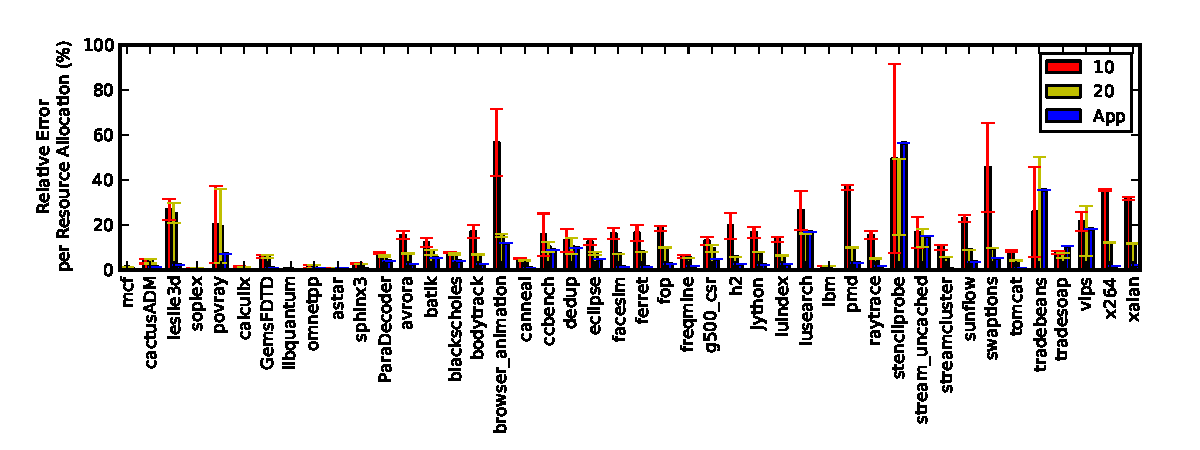
\includegraphics[width=\textwidth]{model_accuracy.pdf}
		\caption{L1 Norm of Relative Error of Response-Time model predicted runtime vs. actual runtime.  Data is from 3 complete trials.}
		\label{fig:model_accuracy}
	\end{center}
\end{figure*}
\begin{figure*}[!t]
	\begin{center}	
%		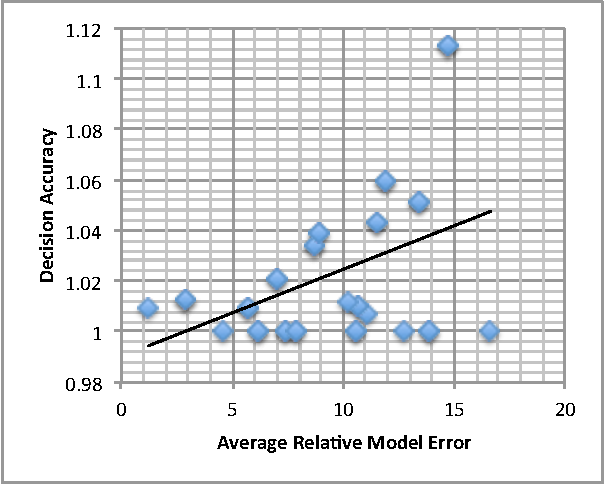
\includegraphics[width=.45\textwidth]{cluster_decision_accuracy.pdf}
%		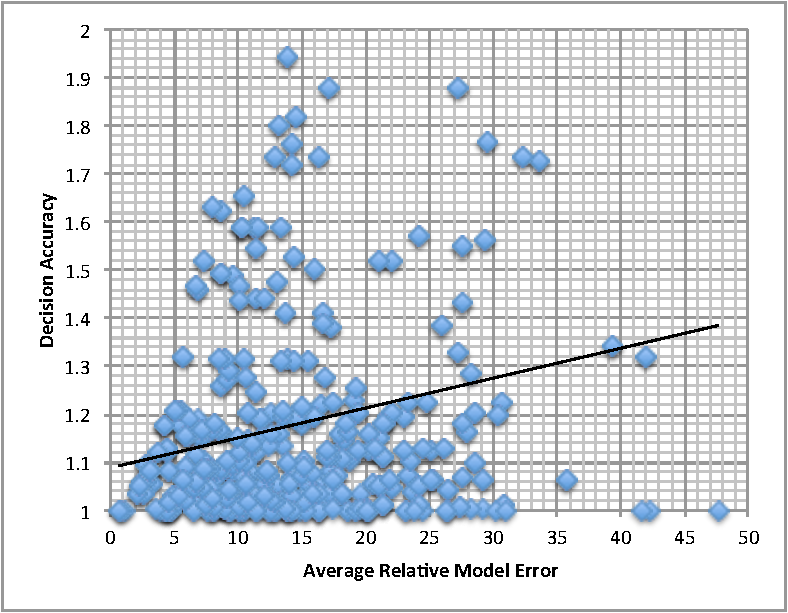
\includegraphics[width=.45\textwidth]{parsec_decision_accuracy.pdf}
		\caption{}
		\label{fig:model_accuracy}
	\end{center}
\end{figure*}


\subsubsection{Resource Allocation Decisions}
\begin{figure*}[!t]
	\begin{center}	
%		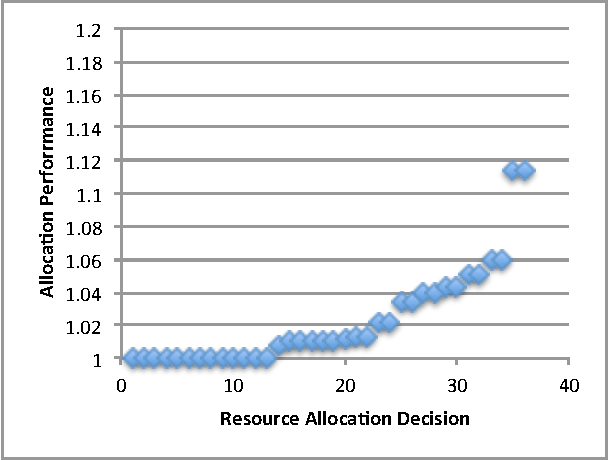
\includegraphics[width=.45\textwidth]{cluster_decision_points.pdf}
%		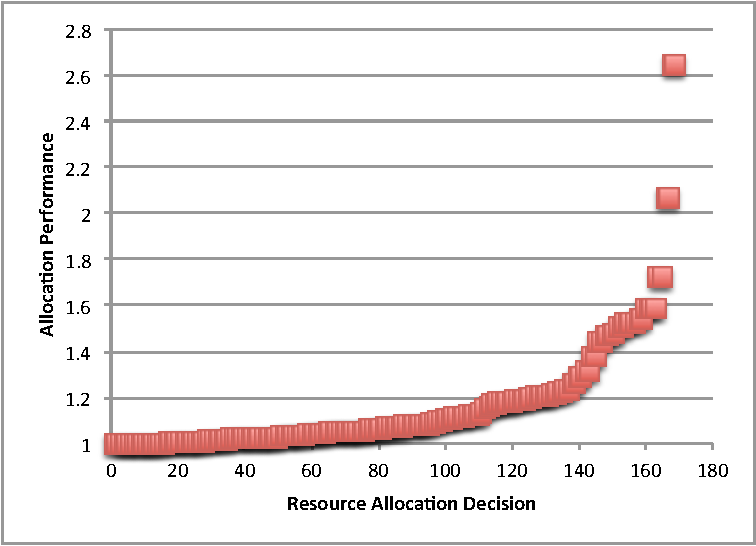
\includegraphics[width=.45\textwidth]{parsec_decision_points.pdf}
		\caption{}
		\label{fig:model_accuracy}
	\end{center}
\end{figure*}



\subsection{Manycore OS Implementation}

\subsubsection{Description of Workloads}


\subsubsection{Response-Time Functions}

\subsubsection{Resource Allocation Decisions}











%In addition, we use a FitPC external multimeter to measure the power
%consumed at the wall socket by the entire system, at a
%\wunits{1}{second} granularity.
%%Total system power is generally between \wunits{185}{W} and \wunits{240}{W}.
%The system-level values
%are correlated with data collected from the hardware energy counters
%using time stamps.  We observed less than one second of delay in these
%measurements consistently across all experiments.  Together, these
%mechanisms allow us to collect accurate energy readings over the
%entire course of an application's execution.
